\RequirePackage{fix-cm}
\documentclass[10pt,letterpaper]{article}
\usepackage[margin=0.65in]{geometry}
\usepackage[T1]{fontenc}
\usepackage{amsmath,amssymb,graphicx,booktabs,longtable,url,array,needspace,placeins}
\usepackage[hidelinks]{hyperref}
\setlength{\emergencystretch}{2em}\setlength{\parindent}{0pt}\setlength{\parskip}{5pt}
\renewcommand{\thesection}{S\arabic{section}}
\renewcommand{\thesubsection}{\thesection.\arabic{subsection}}
\renewcommand{\thefigure}{S\arabic{figure}}
\newcommand{\cival}[3]{\shortstack[r]{#1\\{\fontsize{8.5}{10}\selectfont[#2, #3]}}}
\begin{document}
\begin{center}\Large Supplement to NeST-Com: Fixed-Budget Next-Scale Token Communication\\[4pt]\normalsize Anonymous Authors\end{center}
Algorithms, matched controls and additional results. Full numerical precision, all intervals and technical records accompany this reading edition in the reproduction files.

% Reading-flow navigation 20261103
\textbf{Contents}\par
\begin{tabular}{@{}p{0.47\linewidth}p{0.47\linewidth}@{}}
S1 Algorithms, proofs and implementation (p.~\pageref{sup:1}) & S5 Fixed-policy channel threshold (p.~\pageref{sup:5})\\
S2 System-level results (p.~\pageref{sup:2}) & S6 Qualitative examples and selection (p.~\pageref{sup:6})\\
S3 Matched endpoint and receiver controls (p.~\pageref{sup:3}) & S7 Processing costs and paired quality (p.~\pageref{sup:7})\\
S4 Equal information budgets (p.~\pageref{sup:4}) & S8 Transfer to Kodak24 (p.~\pageref{sup:8})
\end{tabular}


\section{Algorithms and protocol}\label{sup:1}
% Signal and supplement organization 20261103
\textbf{Algorithm overview.} Both terminals configure the frozen MCS and profile directory before transmission. TX obtains scale-wise probabilities, independently terminates each legal token prefix, and fits its arithmetic-code length to the protected body. It sends the selected prefix bitstream with its Profile ID, or a full-budget NULL frame when no source prefix fits. RX recovers the endpoint, independently decodes the prefix, and uses VAR's known-token overwrite and recursive state update for completion. Valid NULL reception and rejected frames both retain their gray outputs in the statistical denominator.

\textbf{Reading map.} S1.1--S1.4 specify the model, coding, frame and calibration; S1.5 gives the fitting algorithm and length proof. S1.6 states verification and statistical assumptions. The companion \path{REPRODUCTION_CHECKLIST.md} links complete configurations, identities, commands and numerical tables. It separates publicly available assets from checkpoints retained in project storage.

\subsection{Representation, models and numerical route}
The tokenizer has a 4096-entry codebook and ten maps of side lengths $(1,2,3,4,5,6,8,10,13,16)$. The VAR-d16 prior uses null class 1000 and greedy prediction, without CFG. Complete coarse maps determine every position's probability in the next map. Both terminals use those known maps; no unreceived same-scale token enters the receiver's entropy context.

The image decoder minimizes MSE+$0.1$ LPIPS on 20\,000 ImageNet training images with a 50/25/25 mixture of continuous latents, fully quantized latents, and interpolated prefix-completed latents. The last input is $F_b+\alpha(F-F_b)$, $\alpha\sim U[0,1]$, with $F_b$ completed from eight source scales. Selection minimizes full-calibration mixture image loss. Tokenizer, prior and codebook remain frozen. The selected decoder is frozen for evaluation.

NeST uses FP32, batch one, eval/no-grad, TF32 off, highest matmul precision, deterministic algorithms and cuDNN deterministic on, with benchmark off. Reproducing the floating-point probability stream requires the recorded numerical route as well as the weights. S7 distinguishes the two physical-core timing protocol from the historical SMT-pair protocol.

Ada retains the pinned LlamaGen-L/VQ16 implementation, predicted ConvNeXt-tiny classes, conditional-branch entropy CDFs and CFG 4/T1/top-$k$2000/top-$p$1 sampled completion. Its 10-bit class is paid. ARPC uses its public 0.06M preset, CFG 3, temperature 0.5 and seed 0; its paid caption and source container are preserved. Latent JSCC uses MSE+$0.1$ LPIPS+$0.01$ latent consistency and shared $D_c$, with 100k updates; SwinJSCC uses RGB MSE, 200k updates and minimum calibration-MSE selection. Both use the fixed 20k training subset. External models retain their own numerical routes rather than inheriting NeST's environment.



\subsection{Integer CDFs and independently terminated prefixes}
FP32 logits pass through \texttt{torch.log\_softmax}; NumPy float64 then performs stable normalization. For vocabulary $V=4096$ and total frequency $M=2^{24}$,
\begin{align*}
p_j&=\frac{\exp(\ell_j-\max_k\ell_k)}{\sum_k\exp(\ell_k-\max_k\ell_k)},&
f_j&=\lfloor p_j(M-V)\rfloor+1,\\
d&=M-\sum_j f_j,&f_{j^*}&\leftarrow f_{j^*}+d,\quad j^*=\arg\max_jp_j.
\end{align*}
Exact ties use the smallest codebook index. The int64 CDF is $[0,\operatorname{cumsum}(f)]$, with strictly positive frequencies. No CDF table is transmitted. The implementation is \path{src/var_comm/entropy.py}.

The arithmetic interval starts at $[0,2^{32}-1]$. An incremental encoder evaluates successive prefixes; each is finalized independently, without changing the incremental state. Finalization emits $b=0$ if low$<2^{30}$, otherwise $b=1$, followed by pending+1 inverse bits. RX initializes a 32-bit state, uses bounded zero extension, and requires exactly 30 terminal zero reads. It re-encodes recovered tokens and requires exact equality to the received payload. The paid Profile ID identifies the endpoint $(m,K)$ in the configured directory and hence the token count. Prefix streams are not slices of a longer codeword. Missing files and invalid model/CDF inputs are execution errors, not receiver successes or valid NULL frames.

\subsection{Digital frame and rejection rules}
The 68-symbol header carries a 12-bit profile, CRC16 and six zero termination bits. Its convolutional encoder has constraint length 7 and octal generators $(171,133)$, rate 1/2; its 68 coded bits are repeated to 136 bits and mapped to 68 rotated-BPSK symbols. Terminated Viterbi decoding requires final state zero. CRC uses polynomial 0x1021, initial 0xFFFF, MSB-first integer fields. The body CRC covers the 13-bit length, source bits and known zero padding.

For $q=\log_2M_{\rm QAM}$, $n=(N-68)q$, $k=\lfloor rn\rfloor$ and source capacity $k-29$. All 12 declared MCSs are constructor-admitted at both budgets. Sionna2.2.0 uses CPU FP32, one 5G-NR LDPC block and RV0: filler shortening, first-$2Z$ and tail puncturing, no repetition. Decoder settings are boxplus-phi/check, sum/variable, flooding, 20 iterations, LLR clipping 20, hard output and information bits returned, PCM pruning on, HARQ and early stopping off. Gray-mapped QAM has nominal $E_s=2$ without per-frame renormalization. Public PCG64 scrambling follows rate matching; RX reverses its LLR signs. The public seed and exact mapping are specified in the companion protocol.

The complete 24 constructor layouts, including base graphs, lifting factors, filler and puncturing counts, are supplied in the companion \path{phy_layouts.csv}.

Profile/header CRC, body CRC, invalid length, padding or arithmetic-canonical failures produce gray RGB 0.5. A valid NULL frame also produces gray and retains the full statistical denominator. If no source prefix fits, TX sends a NULL frame with a two-bit zero payload using the full $N$-symbol budget; its directory entry is the NULL profile. Current directories have seven WHOLE, 651 NeST or 256 Ada source profiles, plus one NULL profile each. Every ID fits in 12 bits without changing the header. Each method/MCS directory is fixed before calibration and shared across all images and target ceilings. Both terminals know the MCS and directory before transmission; the received Profile ID selects only the endpoint. Changing policy requires configuring both terminals before data transmission. Earlier shared catalogues also stored MCS parameters in each profile entry; their identities and experiment associations are distinguished below.

\paragraph{Policy and directory index.}
The policy IDs below distinguish current calibration from earlier experiments. Entries are in WHOLE/NeST/Ada order, with $q=\log_2 M$; a single MCS entry applies to all listed methods. Ceilings $(m,K)$ are target limits, not per-image transmitted endpoints; Ada's ceiling is a token count. Table IV gives current main policies, whereas the experiment index below identifies retained auxiliary configurations.
{\small\setlength{\tabcolsep}{3pt}\begin{longtable}{@{}lllp{4.3cm}l@{}}\toprule
ID & $N$/design SNR & $(q,r)$ & Ceilings W/N/A & Directory W/N/A\\\midrule\endhead
U4 & 1024/4 & 2,2/3 & (7,0) / (7,25) / 256 & U/U/U\\
U7 & 1024/7 & 4,1/2 & (8,0) / (8,0) / 256 & U/U/U\\
U10 & 1024/10 & 4,2/3 & (9,0) / (8,126) / 256 & U/U/U\\
U19 & 1024/19 & $(6,5/6);(6,5/6);(4,5/6)$ & (10,0) / (10,0) / 256 & U/U/U\\
H4 & 1024/4 & 2,2/3 & (7,0) / (7,25) / 256 & HW/HT/HA\\
H7 & 1024/7 & 4,1/2 & (10,0) / (10,0) / 256 & H7/HT/H7\\
H10 & 1024/10 & 4,2/3 & (9,0) / (8,126) / 256 & HW/HT/HA\\
H19 & 1024/19 & 6,5/6 & (10,0) / (10,0) / 256 & HW/HT/HA\\
L4 & 512/4 & 2,2/3 & (6,0) / (5,27) / 256 & LW/LT/LW\\
L10 & 512/10 & 4,2/3 & (7,0) / (7,0) / 256 & LW/LT/LW\\
L19 & 512/19 & 6,5/6 & (8,0) / (8,84) / 256 & LW/LT/LW\\
C1024 & 1024/10 & 4,2/3 & (8,126) & HT\\
C512 & 512/10 & 4,2/3 & (7,0) & LT\\
\bottomrule\end{longtable}}
U denotes the current per-method/MCS directory. HW/HT/HA, H7 and LW/LT identify the earlier endpoint/MCS catalogues; KT adds NULL entries without changing source entries. Exact directory identities are in the companion policy index.
{\small\setlength{\tabcolsep}{3pt}\begin{longtable}{@{}p{6.2cm}p{3.1cm}p{6.0cm}@{}}\toprule
Experiment & Policy IDs & Directory and scope\\\midrule\endhead
Current N1024 common500 and main Fig.3 & U4/U7/U10/U19 & U; Table IV\\
N512 common500 & L4/L10/L19 & LW/LT/LW; Table IV\\
Matched quality grids (S3) & C1024; C512 & HT; LT; only allowed endpoints vary\\
Receiver A0/B0/C0 (S3) & H7/H10/H19, NeST ceiling & HT; Token prefixes; 19 dB is the final-scale structural check\\
Ada sampling/argmax (S3) & L4/L10/H10, Ada ceiling & LW/LW/HA; identical received prefixes\\
Equal information budgets (S4) & No MCS; ceilings (10,0)/(10,0)/256 & Information-packet protocol; no PHY\\
Fixed 10-dB threshold test (S5) & H10 at actual 8--10 dB & HW/HT/HA; fixed transmitted frames\\
Additional image examples & H7/H10 & S6/companion; main Fig.3 uses U10\\
Corrected-resource and compiled32 timing (S7) & H10 & HW/HT/HA; compiled32 uses Ada entry\\
Matched-grid timing (S7) & C1024 & Whole: HW; other grids: HT\\
Historical timing & H7/H10/L10 & Companion only; separate SMT protocol\\
Kodak24 (S8) & H4/H10/H19 & WHOLE/Quarter: HW; Token: KT; Ada: HA\\
\bottomrule\end{longtable}}
For Kodak, Quarter and Token share the NeST ceiling but use their respective endpoint grids. Receiver-only interventions reuse their original decoded prefixes. U10 and H10 have identical MCSs and target ceilings, so the H10 timing and threshold studies probe the same modulation/coding and source-limit choices; their distinct directory versions identify the actual frames used. At 19 dB, historical Ada H19 uses 64-QAM rate 5/6, while current U19 uses 16-QAM rate 5/6. Kodak therefore evaluates the historical frozen configurations. External-system manifests identify their unchanged configurations.

\subsection{Candidate pools and calibration}
At N1024, all three token families use the same 12 MCSs, $q\in\{2,4,6\}$ and $r\in\{1/2,2/3,3/4,5/6\}$. WHOLE has seven complete-scale target ceilings. NeST searches the 25 Quarter target ceilings and permits every integer endpoint up to each target. Ada has the maximum target of 256 and permits every shorter positive prefix. This gives 84/300/12 candidates for WHOLE/NeST/Ada, respectively. Equal MCS and selection rules do not mean identical endpoint grammars. NeST's search is finite over 25 ceilings, not an exhaustive search over all 651 possible ceilings.

Each candidate uses the same fixed 100 calibration sources with one channel realization (seed 4101) at 4/7/10/19 dB. Per family/SNR, the top three plus the predetermined maximum-ceiling QPSK rate-1/2 anchor advance, with duplicate candidate IDs removed. Final confirmation uses all 1000 calibration sources and three realizations (4101/4102/4103). Source-level means of DINOv2-L cosine include gray failures and valid NULL frames; their equal-weight mean is maximized. Ties use a fixed lexical candidate-ID order. Identical actual streams or receiver inputs may be reused after full identity checks while all candidate logical positions remain in the denominator. The original serial Ada quality implementation, FP32/TF32-off configuration, CFG 4, T1, top-k 2000 and top-p 1 are fixed before evaluation.

No common500 result participates in policy selection. Frozen policies are then evaluated on 500 sources, three actual channel realizations per source (6201/6202/6203). The original N512 calibration and its inherited Token refinement remain unchanged; the new matched N512 diagnostic below instead holds every factor except the termination grid fixed. Kodak, threshold and historical receiver diagnostics retain their specifically identified earlier policies.




DINOv2 is the policy objective. DISTS, DreamSim and CLIP-I are feature-based source-reference measures; their agreement is not independent human perceptual validation. Source-bit capacity utilization excludes paid body fields and is not total air-interface efficiency. Ada may transmit all 256 tokens and leave capacity unused. N512 and N1024 are separately calibrated systems, not a budget-only causal intervention.

\Needspace{20\baselineskip}\subsection{Actual-length fitting and length property}
For each complete scale, the prior evaluates the probability map from known coarser maps. Raster tokens enter one shared incremental arithmetic encoder. At every allowed endpoint, a non-mutating finish produces a separate terminated stream. The current measured path is:
\begin{enumerate}
\item Fix MCS, public directory, legal endpoint grid and calibrated ceiling. Order endpoints by retained token count.
\item Traverse source tokens once, sharing scale-wise probability evaluation and incremental coding. At each allowed endpoint obtain an independently terminated prefix without changing encoder state.
\item Compare every allowed candidate's terminated arithmetic-code length with the source-bit capacity. For NeST/WHOLE require $b+29\le k$; Ada additionally pays its 10-bit class.
\item Select the most-token feasible endpoint below the ceiling. Transmit its entire prefix bitstream and Profile ID; if none fits, transmit the full-budget NULL frame.
\item Recover the profile and then independently decode the corresponding body. Rejected frames and valid NULL frames both retain gray outputs in every metric denominator.
\end{enumerate}
For Quarter/Eighth, boundary counts are $\lfloor jL/d\rfloor$, $j=1,\ldots,d-1$, $d=4/8$, with duplicates removed and complete boundaries included. Token includes every integer boundary count. No partial stream is obtained by cutting a longer finalized stream.

Let $E$ be emitted bits and $P$ pending underflow bits. The original coder's finalization yields $b=E+P+2$. Every E1/E2 renormalization emits $P+1$ bits and clears $P$, and every E3 increments $P$; each raises $E+P$ by one. A token's interval update alone leaves it unchanged. Thus independently terminated lengths along this shared path are nondecreasing, with possible ties. Integer reference checks and the existing source streams verify this coder-specific identity and non-mutating finalization. The measured implementation still constructs and scans all allowed candidates; candidate comparisons do not add prior forward passes. The reported timings include this full scan.

\subsection{Verification and statistical units}
Integer reference vectors verify positive frequencies, frequency totals, deterministic ties, independent termination/decoding and rejection of noncanonical appended bits. Two real-model vectors check independently reconstructed CDFs and recovered tokens:
{\small\setlength{\tabcolsep}{3pt}\begin{longtable}{@{}llrrrr@{}}\toprule
Vector & $(m,K)$ & Tokens & Source bits & CDF scales & Exact TX/RX\\\midrule\endhead
Whole & (4, 0) & 30 & 318 & 4 & yes\\
Boundary & (6, 34) & 125 & 1241 & 7 & yes\\
\bottomrule\end{longtable}}
RX uses no TX probability table, unsent token or hidden source state. These checks establish correct decoding under the specified numerical route; heterogeneous-device CDF interchangeability is not claimed. Commands and complete verification records are in the companion.

Common500 uses its original 10\,000$\times500$ source-bootstrap bank; controls use a separately ordered 10\,000$\times100$ bank. Kodak uses the existing 10\,000$\times24$ bank. Each source first averages its three events, then receives equal weight; paired differences precede resampling. Full source IDs, pixel hashes and native receiver identities control reuse. No simultaneous multiplicity-adjusted interval claim is made.

\section{System-level results}\label{sup:2}
The $N=1024$ WHOLE/NeST/Ada results use unified calibration. Latent JSCC, SwinJSCC, BPG and the ARPC digital adaptation retain their original outputs and configurations. All results use 500 test images and three channel realizations per image. The three calibrated token methods share noise; external methods retain their original noise identities. Pairing across systems is by source. $N=512$ is independently calibrated; Quarter denotes the earlier quarter-grid system, while NeST uses token-level fallback.

ARPC is a progressive source codec coupled here to the specified protected digital link, using its public 0.06M preset, CFG 3, temperature 0.5 and paid caption/container. This comparison concerns that adaptation. Lower DISTS, DreamSim and LPIPS, and higher PSNR and CLIP-I, are favorable. Means below retain every operating point; complete pointwise intervals and every external paired comparison remain in the companion CSVs.
\begin{figure}[htbp]\centering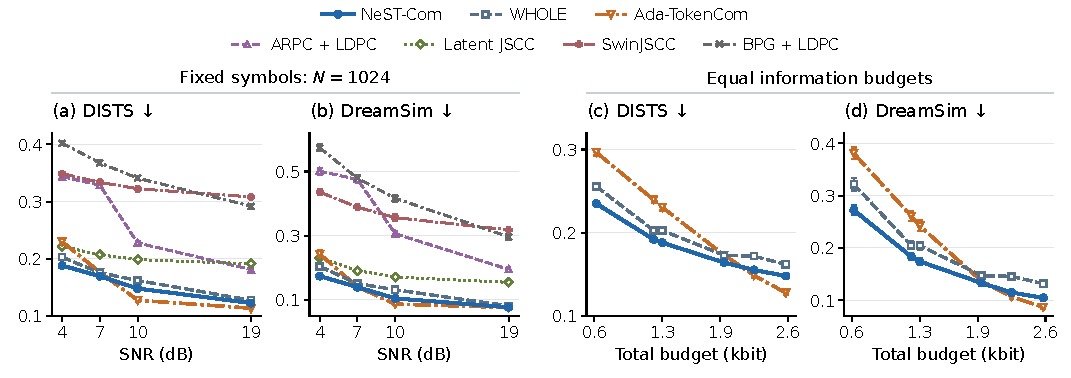
\includegraphics[width=\linewidth]{figures/figure2_complete_with_arpc.pdf}
\caption{System-level and equal-information-budget comparisons, including the ARPC digital adaptation. All 92 points and pointwise 95\% source-bootstrap intervals are retained. Ada denotes the predicted-class, fixed-frame adaptation.}\label{fig:complete_comparison}\end{figure}

\textbf{$N=1024$ source means (PSNR in dB).}\par
{\small\setlength{\tabcolsep}{3pt}\renewcommand{\arraystretch}{1.08}
\begin{longtable}{@{}llrrrrr@{}}\toprule
SNR & Method & PSNR $\uparrow$ & DISTS $\downarrow$ & DreamSim $\downarrow$ & LPIPS $\downarrow$ & CLIP-I $\uparrow$\\\midrule\endhead
4 & ARPC & 14.184 & 0.3436 & 0.5010 & 0.5124 & 0.6442\\*
4 & Ada & 13.332 & 0.2300 & 0.2431 & 0.3952 & 0.8280\\*
4 & BPG & 20.743 & 0.4022 & 0.5737 & 0.7255 & 0.5859\\*
4 & Latent & 19.658 & 0.2218 & 0.2317 & 0.2188 & 0.7408\\*
4 & NeST & 17.649 & 0.1886 & 0.1749 & 0.2554 & 0.8269\\*
4 & Swin & 21.671 & 0.3488 & 0.4359 & 0.5297 & 0.6267\\*
4 & WHOLE & 16.832 & 0.2028 & 0.2046 & 0.2878 & 0.8077\\
7 & ARPC & 14.759 & 0.3287 & 0.4751 & 0.4809 & 0.6508\\*
7 & Ada & 15.929 & 0.1778 & 0.1421 & 0.2706 & 0.8591\\*
7 & BPG & 21.717 & 0.3676 & 0.4788 & 0.6500 & 0.6150\\*
7 & Latent & 20.369 & 0.2070 & 0.1912 & 0.1893 & 0.7717\\*
7 & NeST & 19.006 & 0.1671 & 0.1369 & 0.2058 & 0.8549\\*
7 & Swin & 22.475 & 0.3336 & 0.3887 & 0.4933 & 0.6505\\*
7 & WHOLE & 18.508 & 0.1774 & 0.1528 & 0.2243 & 0.8450\\
10 & ARPC & 16.471 & 0.2278 & 0.3062 & 0.3413 & 0.7134\\*
10 & Ada & 19.559 & 0.1275 & 0.0871 & 0.1674 & 0.8841\\*
10 & BPG & 22.543 & 0.3409 & 0.4165 & 0.5894 & 0.6350\\*
10 & Latent & 20.803 & 0.1986 & 0.1712 & 0.1733 & 0.7892\\*
10 & NeST & 20.194 & 0.1481 & 0.1048 & 0.1658 & 0.8769\\*
10 & Swin & 23.026 & 0.3224 & 0.3564 & 0.4687 & 0.6691\\*
10 & WHOLE & 19.313 & 0.1621 & 0.1317 & 0.1987 & 0.8577\\
19 & ARPC & 18.199 & 0.1812 & 0.1952 & 0.2503 & 0.7880\\*
19 & Ada & 20.934 & 0.1136 & 0.0763 & 0.1377 & 0.8924\\*
19 & BPG & 24.230 & 0.2920 & 0.2964 & 0.4584 & 0.6843\\*
19 & Latent & 21.245 & 0.1911 & 0.1546 & 0.1585 & 0.8041\\*
19 & NeST & 22.334 & 0.1226 & 0.0772 & 0.1151 & 0.9015\\*
19 & Swin & 23.698 & 0.3081 & 0.3179 & 0.4400 & 0.6966\\*
19 & WHOLE & 21.844 & 0.1274 & 0.0815 & 0.1234 & 0.8969\\
\bottomrule\end{longtable}}
\Needspace{18\baselineskip}
\textbf{$N=512$ source means (PSNR in dB).}\par
{\small\setlength{\tabcolsep}{3pt}\renewcommand{\arraystretch}{1.08}
\begin{longtable}{@{}llrrrrr@{}}\toprule
SNR & Method & PSNR $\uparrow$ & DISTS $\downarrow$ & DreamSim $\downarrow$ & LPIPS $\downarrow$ & CLIP-I $\uparrow$\\\midrule\endhead
4 & Ada & 11.318 & 0.2996 & 0.3847 & 0.5542 & 0.7892\\*
4 & WHOLE & 15.107 & 0.2580 & 0.3247 & 0.3951 & 0.7469\\*
4 & NeST & 15.611 & 0.2363 & 0.2740 & 0.3565 & 0.7691\\*
4 & Quarter & 15.499 & 0.2406 & 0.2819 & 0.3652 & 0.7657\\
10 & Ada & 13.165 & 0.2367 & 0.2582 & 0.4110 & 0.8257\\*
10 & WHOLE & 16.821 & 0.2030 & 0.2049 & 0.2881 & 0.8074\\*
10 & NeST & 17.413 & 0.1922 & 0.1837 & 0.2650 & 0.8211\\*
10 & Quarter & 17.220 & 0.1958 & 0.1922 & 0.2726 & 0.8150\\
19 & Ada & 17.690 & 0.1496 & 0.1078 & 0.2146 & 0.8723\\*
19 & WHOLE & 18.638 & 0.1718 & 0.1458 & 0.2175 & 0.8484\\*
19 & NeST & 19.632 & 0.1554 & 0.1150 & 0.1832 & 0.8689\\*
19 & Quarter & 19.430 & 0.1587 & 0.1217 & 0.1901 & 0.8640\\
\bottomrule\end{longtable}}
At $N=1024$, 10 dB, Ada has lower mean DISTS and DreamSim than NeST, while SwinJSCC and BPG have higher PSNR. NeST's gains over WHOLE and its metric-dependent differences from Ada are quantified below. ARPC's values describe the specified digital adaptation rather than its compression performance independent of the link.
\textbf{Direct paired comparisons.} Every cell below is the first method minus the second, with its 95\% source-paired interval. These contrasts retain both favorable and unfavorable results; differences of marginal intervals are not used.

{\small\setlength{\tabcolsep}{3pt}\renewcommand{\arraystretch}{1.08}
\begin{longtable}{@{}lllrrrrr@{}}\toprule
$N$ & SNR & Difference & PSNR $\uparrow$ & DISTS $\downarrow$ & DreamSim $\downarrow$ & LPIPS $\downarrow$ & CLIP-I $\uparrow$\\\midrule\endhead
512 & 4 & NeST-Ada & \cival{+4.293}{4.098}{4.492} & \cival{-0.0633}{-0.0677}{-0.0589} & \cival{-0.1107}{-0.1221}{-0.0996} & \cival{-0.1976}{-0.2052}{-0.1901} & \cival{-0.0201}{-0.0284}{-0.0117}\\*
512 & 4 & NeST-WHOLE & \cival{+0.504}{0.440}{0.573} & \cival{-0.0217}{-0.0245}{-0.0190} & \cival{-0.0506}{-0.0566}{-0.0445} & \cival{-0.0386}{-0.0428}{-0.0345} & \cival{+0.0222}{0.0171}{0.0274}\\*
512 & 4 & WHOLE-Ada & \cival{+3.788}{3.583}{3.998} & \cival{-0.0416}{-0.0467}{-0.0364} & \cival{-0.0601}{-0.0733}{-0.0471} & \cival{-0.1590}{-0.1682}{-0.1499} & \cival{-0.0423}{-0.0511}{-0.0335}\\
512 & 10 & NeST-Ada & \cival{+4.248}{4.071}{4.428} & \cival{-0.0446}{-0.0476}{-0.0415} & \cival{-0.0744}{-0.0829}{-0.0658} & \cival{-0.1460}{-0.1515}{-0.1406} & \cival{-0.0047}{-0.0114}{0.0019}\\*
512 & 10 & NeST-WHOLE & \cival{+0.592}{0.544}{0.643} & \cival{-0.0108}{-0.0118}{-0.0099} & \cival{-0.0211}{-0.0236}{-0.0186} & \cival{-0.0231}{-0.0245}{-0.0216} & \cival{+0.0136}{0.0101}{0.0172}\\*
512 & 10 & WHOLE-Ada & \cival{+3.657}{3.481}{3.835} & \cival{-0.0337}{-0.0369}{-0.0306} & \cival{-0.0533}{-0.0623}{-0.0444} & \cival{-0.1229}{-0.1286}{-0.1174} & \cival{-0.0183}{-0.0255}{-0.0113}\\
512 & 19 & NeST-Ada & \cival{+1.942}{1.778}{2.110} & \cival{+0.0058}{0.0036}{0.0079} & \cival{+0.0072}{0.0037}{0.0106} & \cival{-0.0313}{-0.0347}{-0.0281} & \cival{-0.0034}{-0.0082}{0.0013}\\*
512 & 19 & NeST-WHOLE & \cival{+0.994}{0.940}{1.048} & \cival{-0.0164}{-0.0175}{-0.0154} & \cival{-0.0308}{-0.0333}{-0.0284} & \cival{-0.0343}{-0.0358}{-0.0328} & \cival{+0.0205}{0.0170}{0.0242}\\*
512 & 19 & WHOLE-Ada & \cival{+0.948}{0.778}{1.124} & \cival{+0.0223}{0.0199}{0.0246} & \cival{+0.0380}{0.0338}{0.0421} & \cival{+0.0030}{-0.0007}{0.0065} & \cival{-0.0239}{-0.0291}{-0.0189}\\
1024 & 4 & NeST-ARPC & \cival{+3.465}{3.322}{3.612} & \cival{-0.1549}{-0.1595}{-0.1505} & \cival{-0.3261}{-0.3363}{-0.3158} & \cival{-0.2570}{-0.2636}{-0.2506} & \cival{+0.1827}{0.1747}{0.1908}\\*
1024 & 4 & NeST-Ada & \cival{+4.317}{4.123}{4.518} & \cival{-0.0414}{-0.0446}{-0.0381} & \cival{-0.0682}{-0.0760}{-0.0604} & \cival{-0.1398}{-0.1454}{-0.1343} & \cival{-0.0012}{-0.0074}{0.0049}\\*
1024 & 4 & NeST-WHOLE & \cival{+0.817}{0.760}{0.877} & \cival{-0.0142}{-0.0155}{-0.0127} & \cival{-0.0297}{-0.0330}{-0.0264} & \cival{-0.0324}{-0.0342}{-0.0304} & \cival{+0.0192}{0.0153}{0.0230}\\*
1024 & 4 & WHOLE-Ada & \cival{+3.500}{3.312}{3.695} & \cival{-0.0272}{-0.0304}{-0.0240} & \cival{-0.0385}{-0.0472}{-0.0301} & \cival{-0.1074}{-0.1132}{-0.1017} & \cival{-0.0203}{-0.0271}{-0.0139}\\
1024 & 7 & NeST-ARPC & \cival{+4.247}{4.108}{4.390} & \cival{-0.1616}{-0.1659}{-0.1572} & \cival{-0.3383}{-0.3480}{-0.3284} & \cival{-0.2751}{-0.2806}{-0.2696} & \cival{+0.2042}{0.1964}{0.2120}\\*
1024 & 7 & NeST-Ada & \cival{+3.077}{2.881}{3.281} & \cival{-0.0107}{-0.0149}{-0.0067} & \cival{-0.0052}{-0.0116}{0.0010} & \cival{-0.0648}{-0.0702}{-0.0594} & \cival{-0.0041}{-0.0095}{0.0011}\\*
1024 & 7 & NeST-WHOLE & \cival{+0.498}{0.441}{0.553} & \cival{-0.0103}{-0.0139}{-0.0068} & \cival{-0.0159}{-0.0207}{-0.0112} & \cival{-0.0186}{-0.0228}{-0.0144} & \cival{+0.0099}{0.0065}{0.0135}\\*
1024 & 7 & WHOLE-Ada & \cival{+2.579}{2.378}{2.788} & \cival{-0.0004}{-0.0046}{0.0037} & \cival{+0.0107}{0.0044}{0.0171} & \cival{-0.0462}{-0.0518}{-0.0408} & \cival{-0.0141}{-0.0197}{-0.0085}\\
1024 & 10 & NeST-ARPC & \cival{+3.723}{3.615}{3.835} & \cival{-0.0797}{-0.0822}{-0.0772} & \cival{-0.2014}{-0.2090}{-0.1939} & \cival{-0.1755}{-0.1788}{-0.1722} & \cival{+0.1636}{0.1562}{0.1708}\\*
1024 & 10 & NeST-Ada & \cival{+0.635}{0.521}{0.753} & \cival{+0.0205}{0.0189}{0.0222} & \cival{+0.0177}{0.0153}{0.0199} & \cival{-0.0016}{-0.0041}{0.0008} & \cival{-0.0072}{-0.0114}{-0.0031}\\*
1024 & 10 & NeST-WHOLE & \cival{+0.881}{0.808}{0.956} & \cival{-0.0141}{-0.0153}{-0.0128} & \cival{-0.0270}{-0.0299}{-0.0241} & \cival{-0.0329}{-0.0356}{-0.0302} & \cival{+0.0192}{0.0155}{0.0231}\\*
1024 & 10 & WHOLE-Ada & \cival{-0.246}{-0.371}{-0.118} & \cival{+0.0346}{0.0327}{0.0365} & \cival{+0.0446}{0.0409}{0.0484} & \cival{+0.0314}{0.0279}{0.0348} & \cival{-0.0264}{-0.0315}{-0.0215}\\
1024 & 19 & NeST-ARPC & \cival{+4.135}{4.040}{4.228} & \cival{-0.0586}{-0.0608}{-0.0564} & \cival{-0.1180}{-0.1237}{-0.1124} & \cival{-0.1352}{-0.1385}{-0.1321} & \cival{+0.1135}{0.1070}{0.1199}\\*
1024 & 19 & NeST-Ada & \cival{+1.400}{1.340}{1.459} & \cival{+0.0090}{0.0076}{0.0104} & \cival{+0.0009}{-0.0009}{0.0028} & \cival{-0.0226}{-0.0236}{-0.0215} & \cival{+0.0091}{0.0053}{0.0130}\\*
1024 & 19 & NeST-WHOLE & \cival{+0.490}{0.457}{0.523} & \cival{-0.0048}{-0.0053}{-0.0043} & \cival{-0.0043}{-0.0051}{-0.0036} & \cival{-0.0082}{-0.0087}{-0.0078} & \cival{+0.0046}{0.0030}{0.0062}\\*
1024 & 19 & WHOLE-Ada & \cival{+0.910}{0.860}{0.961} & \cival{+0.0138}{0.0125}{0.0152} & \cival{+0.0052}{0.0034}{0.0070} & \cival{-0.0143}{-0.0153}{-0.0133} & \cival{+0.0045}{0.0008}{0.0083}\\
\bottomrule\end{longtable}}

\textbf{Source-bit utilization (\%) / gray outputs out of 1500, $N=1024$.}\par
{\small\setlength{\tabcolsep}{3pt}\renewcommand{\arraystretch}{1.08}
\begin{longtable}{@{}lrrr@{}}\toprule
SNR & WHOLE & NeST & Ada\\\midrule\endhead
4 & 73.81 / 0 & 99.56 / 1 & 99.56 / 0\\
7 & 83.19 / 11 & 99.71 / 7 & 99.67 / 10\\
10 & 77.70 / 0 & 99.79 / 0 & 98.72 / 0\\
19 & 85.24 / 0 & 99.83 / 0 & 87.38 / 0\\
\bottomrule\end{longtable}}
No valid NULL frame occurs in these cells; the listed gray outputs are rejected receptions. BPG has 11 body-CRC rejections across the four SNRs, while the other reused external methods have none. All failures stay in the denominator. Source-level better/tie/worse counts and their full distributions are supplied as CSVs; aggregate gains do not imply improvement for every image.
\section{Matched Endpoint and Receiver Controls}\label{sup:3}
These controls use the same fixed 100 source images and three shared noise realizations per image. They isolate termination granularity or receiver use of a fixed received prefix; they do not decompose the independently calibrated 500-image system gains. All differences are source-paired, with 95\% intervals.
\subsection{Matched termination grids}
At $N=1024$, 10 dB, all four grids share 16-QAM rate 2/3, ceiling $(8,126)$, model and receiver. At $N=512$, 10 dB, the same factors are held fixed with ceiling $(7,0)$. Only allowed termination points change. The complete-scale control has five/four endpoints at the respective budgets; it is not replaced by the separately calibrated WHOLE policy.

{\small\setlength{\tabcolsep}{3pt}\renewcommand{\arraystretch}{1.08}
\begin{longtable}{@{}lrrrrrrr@{}}\toprule
$N$ & Grid & Util. (\%) & PSNR $\uparrow$ & DISTS $\downarrow$ & DreamSim $\downarrow$ & LPIPS $\downarrow$ & CLIP-I $\uparrow$\\\midrule\endhead
1024 & Whole & 78.13 & 19.543 & 0.1650 & 0.1387 & 0.1992 & 0.8456\\
1024 & Quarter & 95.19 & 20.195 & 0.1535 & 0.1143 & 0.1717 & 0.8624\\
1024 & Eighth & 97.44 & 20.301 & 0.1516 & 0.1137 & 0.1687 & 0.8639\\
1024 & Token & 99.85 & 20.367 & 0.1505 & 0.1115 & 0.1665 & 0.8690\\
512 & Whole & 79.18 & 17.015 & 0.2070 & 0.2181 & 0.2915 & 0.7946\\
512 & Quarter & 93.16 & 17.404 & 0.1989 & 0.2018 & 0.2759 & 0.8013\\
512 & Eighth & 96.24 & 17.479 & 0.1974 & 0.1989 & 0.2725 & 0.8049\\
512 & Token & 99.54 & 17.549 & 0.1959 & 0.1933 & 0.2694 & 0.8103\\
\bottomrule\end{longtable}}

{\small\setlength{\tabcolsep}{3pt}\renewcommand{\arraystretch}{1.08}
\begin{longtable}{@{}llrrrrr@{}}\toprule
$N$ & Difference & PSNR $\uparrow$ & DISTS $\downarrow$ & DreamSim $\downarrow$ & LPIPS $\downarrow$ & CLIP-I $\uparrow$\\\midrule\endhead
512 & Eighth-Whole & \cival{+0.464}{0.383}{0.547} & \cival{-0.0096}{-0.0116}{-0.0076} & \cival{-0.0192}{-0.0243}{-0.0138} & \cival{-0.0190}{-0.0222}{-0.0159} & \cival{+0.0103}{0.0023}{0.0179}\\*
512 & Token-Eighth & \cival{+0.070}{0.029}{0.115} & \cival{-0.0015}{-0.0032}{0.0002} & \cival{-0.0056}{-0.0096}{-0.0016} & \cival{-0.0031}{-0.0051}{-0.0012} & \cival{+0.0054}{-0.0006}{0.0114}\\*
512 & Token-Whole & \cival{+0.534}{0.446}{0.625} & \cival{-0.0111}{-0.0134}{-0.0089} & \cival{-0.0248}{-0.0307}{-0.0188} & \cival{-0.0221}{-0.0255}{-0.0187} & \cival{+0.0157}{0.0075}{0.0237}\\
1024 & Eighth-Quarter & \cival{+0.106}{0.068}{0.147} & \cival{-0.0019}{-0.0028}{-0.0011} & \cival{-0.0006}{-0.0020}{0.0008} & \cival{-0.0030}{-0.0041}{-0.0019} & \cival{+0.0016}{-0.0014}{0.0046}\\*
1024 & Eighth-Whole & \cival{+0.757}{0.596}{0.931} & \cival{-0.0134}{-0.0162}{-0.0106} & \cival{-0.0251}{-0.0322}{-0.0185} & \cival{-0.0305}{-0.0367}{-0.0244} & \cival{+0.0183}{0.0098}{0.0274}\\*
1024 & Quarter-Whole & \cival{+0.652}{0.509}{0.807} & \cival{-0.0115}{-0.0141}{-0.0090} & \cival{-0.0245}{-0.0316}{-0.0179} & \cival{-0.0275}{-0.0333}{-0.0219} & \cival{+0.0168}{0.0081}{0.0260}\\*
1024 & Token-Eighth & \cival{+0.066}{0.034}{0.101} & \cival{-0.0011}{-0.0020}{-0.0002} & \cival{-0.0022}{-0.0042}{-0.0001} & \cival{-0.0022}{-0.0032}{-0.0013} & \cival{+0.0051}{0.0002}{0.0105}\\*
1024 & Token-Quarter & \cival{+0.172}{0.125}{0.221} & \cival{-0.0030}{-0.0041}{-0.0020} & \cival{-0.0028}{-0.0050}{-0.0006} & \cival{-0.0052}{-0.0065}{-0.0039} & \cival{+0.0066}{0.0017}{0.0119}\\*
1024 & Token-Whole & \cival{+0.823}{0.659}{1.001} & \cival{-0.0145}{-0.0174}{-0.0117} & \cival{-0.0272}{-0.0342}{-0.0207} & \cival{-0.0327}{-0.0392}{-0.0265} & \cival{+0.0234}{0.0148}{0.0327}\\
\bottomrule\end{longtable}}
Eighth retains about 92\% and 87\% of the Whole-to-Token mean PSNR gains at $N=1024$ and $N=512$, respectively. At $N=1024$, Token improves all five metrics over Eighth in the paired intervals; at $N=512$, the additional DISTS and CLIP-I intervals cross zero. Finer grids therefore provide a quality--processing-cost choice, not a universally optimal endpoint spacing. S7 gives the measured cost of the same $N=1024$ grids; comparisons of cached code lengths are not model-forward counts.
\subsection{Ordered boundary-token interventions}
A0 completes from the prior without the received boundary correction. B0 inserts that correction into the residual while retaining A0's future-condition path. C0 updates both the residual and future conditioning. The actual received prefix, generation settings and failures are held fixed. A0 is not a no-completion baseline, and these ordered differences are not independent additive contributions.

{\small\setlength{\tabcolsep}{3pt}\renewcommand{\arraystretch}{1.08}
\begin{longtable}{@{}llrrrrr@{}}\toprule
SNR & Difference & PSNR $\uparrow$ & DISTS $\downarrow$ & DreamSim $\downarrow$ & LPIPS $\downarrow$ & CLIP-I $\uparrow$\\\midrule\endhead
7 & B0-A0 & \cival{+0.167}{0.139}{0.199} & \cival{-0.0029}{-0.0038}{-0.0020} & \cival{-0.0056}{-0.0077}{-0.0038} & \cival{-0.0064}{-0.0072}{-0.0056} & \cival{-0.0006}{-0.0039}{0.0024}\\*
7 & C0-A0 & \cival{+0.459}{0.394}{0.530} & \cival{-0.0075}{-0.0093}{-0.0058} & \cival{-0.0154}{-0.0198}{-0.0113} & \cival{-0.0172}{-0.0194}{-0.0151} & \cival{+0.0080}{0.0019}{0.0144}\\*
7 & C0-B0 & \cival{+0.292}{0.241}{0.347} & \cival{-0.0046}{-0.0062}{-0.0029} & \cival{-0.0097}{-0.0134}{-0.0063} & \cival{-0.0108}{-0.0127}{-0.0089} & \cival{+0.0086}{0.0028}{0.0151}\\
10 & B0-A0 & \cival{+0.287}{0.240}{0.335} & \cival{-0.0062}{-0.0077}{-0.0048} & \cival{-0.0113}{-0.0147}{-0.0083} & \cival{-0.0123}{-0.0145}{-0.0101} & \cival{+0.0019}{-0.0031}{0.0073}\\*
10 & C0-A0 & \cival{+0.823}{0.659}{1.001} & \cival{-0.0145}{-0.0174}{-0.0117} & \cival{-0.0272}{-0.0342}{-0.0207} & \cival{-0.0327}{-0.0392}{-0.0265} & \cival{+0.0234}{0.0148}{0.0327}\\*
10 & C0-B0 & \cival{+0.537}{0.404}{0.682} & \cival{-0.0083}{-0.0102}{-0.0065} & \cival{-0.0159}{-0.0205}{-0.0116} & \cival{-0.0204}{-0.0252}{-0.0160} & \cival{+0.0215}{0.0139}{0.0296}\\
\bottomrule\end{longtable}}
At $N=1024$, 19 dB, the received boundary lies on the last scale (or the representation is complete). B0 and C0 then use the identical final residual map: no finer-scale conditioning contribution remains.
\subsection{Ada completion sensitivity}
Under the auxiliary configurations in S1.3, only the unreceived-tail choice changes from sampling to argmax. The same 100 sources, paid classes, received prefixes, three original channel outcomes, weights, CFG and precision are retained. Greedy generation rebuilds and updates its own context; it does not reuse the sampled tail. The entropy CDF is unchanged. Full-prefix and gray outputs retain their original treatment. The table gives argmax minus sampling; DISTS was not part of this four-metric diagnostic.

{\small\setlength{\tabcolsep}{3pt}\renewcommand{\arraystretch}{1.08}
\begin{longtable}{@{}llrrrr@{}}\toprule
$N$ & SNR & PSNR $\uparrow$ & DreamSim $\downarrow$ & LPIPS $\downarrow$ & CLIP-I $\uparrow$\\\midrule\endhead
512 & 4 & \cival{-0.475}{-0.801}{-0.152} & \cival{+0.0450}{0.0282}{0.0621} & \cival{+0.0423}{0.0294}{0.0555} & \cival{-0.0261}{-0.0378}{-0.0143}\\
512 & 10 & \cival{-0.651}{-0.984}{-0.338} & \cival{+0.0345}{0.0232}{0.0461} & \cival{+0.0296}{0.0201}{0.0394} & \cival{-0.0231}{-0.0337}{-0.0128}\\
1024 & 10 & \cival{-0.156}{-0.369}{0.057} & \cival{+0.0036}{0.0010}{0.0060} & \cival{+0.0038}{0.0007}{0.0071} & \cival{-0.0013}{-0.0052}{0.0025}\\
\bottomrule\end{longtable}}
Argmax increases both LPIPS and DreamSim at all three points. The main curves retain sampling; the sensitivity result is tied to these auxiliary policies and does not replace the current calibration.
\section{Equal information budgets}\label{sup:4}
Total information budgets are 620, 1212, 1302, 1940, 2248 and 2577 bits. They include 57 common profile/CRC/length bits and another 10 class bits for Ada; arithmetic-code capacities are $B-57$ and $B-67$, respectively. WHOLE/NeST share ceiling $(10,0)$ and Ada permits 1--256 tokens. Independent source reception is error-free, with no PHY or MCS. This removes channel effects but retains tokenizer, prior, class-conditioning and decoder differences.

Each of 500 sources contributes one deterministic WHOLE/NeST reconstruction and three fixed Ada generation repetitions; metric values are averaged within source. These are generation repeats, not channel repeats. All outputs are accepted, with no NULL output. Figure and paired table retain all six budgets.
\begin{figure}[htbp]\centering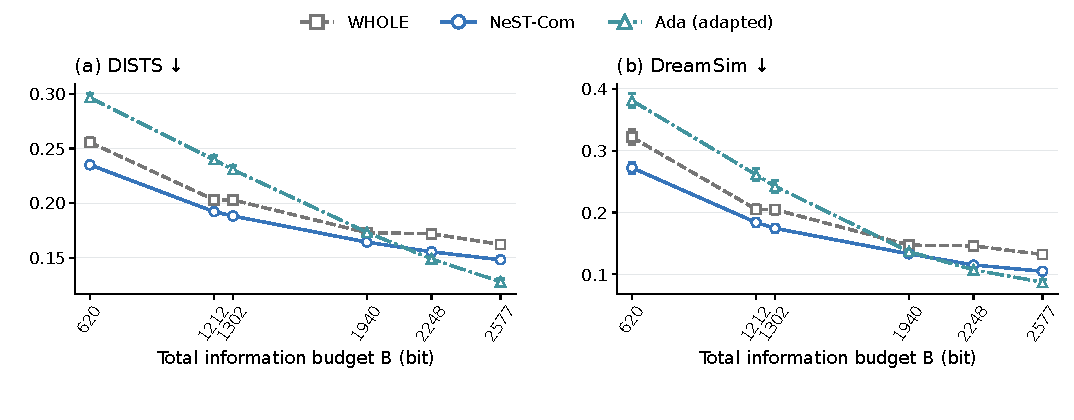
\includegraphics[width=\linewidth]{figures/supp_figure_s1_information_budget.pdf}
\caption{Equal-source means and pointwise 95\% intervals at error-free information budgets, including paid metadata. The numerical spacing of the six budgets is retained.}\label{fig:information-budget}\end{figure}

{\small\setlength{\tabcolsep}{3pt}\renewcommand{\arraystretch}{1.08}
\begin{longtable}{@{}llrrrrr@{}}\toprule
Bits & Difference & PSNR $\uparrow$ & DISTS $\downarrow$ & DreamSim $\downarrow$ & LPIPS $\downarrow$ & CLIP-I $\uparrow$\\\midrule\endhead
620 & NeST-Ada & \cival{+4.271}{4.104}{4.447} & \cival{-0.0616}{-0.0651}{-0.0582} & \cival{-0.1087}{-0.1192}{-0.0982} & \cival{-0.1948}{-0.2016}{-0.1881} & \cival{-0.0192}{-0.0272}{-0.0112}\\*
620 & NeST-WHOLE & \cival{+0.495}{0.431}{0.562} & \cival{-0.0206}{-0.0227}{-0.0185} & \cival{-0.0494}{-0.0553}{-0.0436} & \cival{-0.0376}{-0.0414}{-0.0338} & \cival{+0.0216}{0.0165}{0.0268}\\
1212 & NeST-Ada & \cival{+4.345}{4.172}{4.526} & \cival{-0.0476}{-0.0507}{-0.0446} & \cival{-0.0773}{-0.0853}{-0.0693} & \cival{-0.1479}{-0.1533}{-0.1427} & \cival{-0.0003}{-0.0067}{0.0059}\\*
1212 & NeST-WHOLE & \cival{+0.593}{0.546}{0.644} & \cival{-0.0109}{-0.0119}{-0.0099} & \cival{-0.0212}{-0.0237}{-0.0187} & \cival{-0.0231}{-0.0246}{-0.0217} & \cival{+0.0137}{0.0101}{0.0172}\\
1302 & NeST-Ada & \cival{+4.269}{4.101}{4.443} & \cival{-0.0424}{-0.0453}{-0.0395} & \cival{-0.0680}{-0.0754}{-0.0607} & \cival{-0.1389}{-0.1439}{-0.1339} & \cival{-0.0029}{-0.0086}{0.0025}\\*
1302 & NeST-WHOLE & \cival{+0.824}{0.767}{0.882} & \cival{-0.0147}{-0.0158}{-0.0136} & \cival{-0.0303}{-0.0334}{-0.0273} & \cival{-0.0329}{-0.0345}{-0.0313} & \cival{+0.0195}{0.0157}{0.0233}\\
1940 & NeST-Ada & \cival{+2.978}{2.810}{3.152} & \cival{-0.0091}{-0.0116}{-0.0067} & \cival{-0.0036}{-0.0082}{0.0007} & \cival{-0.0641}{-0.0681}{-0.0603} & \cival{-0.0049}{-0.0096}{-0.0002}\\*
1940 & NeST-WHOLE & \cival{+0.491}{0.452}{0.530} & \cival{-0.0087}{-0.0095}{-0.0079} & \cival{-0.0141}{-0.0157}{-0.0125} & \cival{-0.0168}{-0.0178}{-0.0158} & \cival{+0.0092}{0.0064}{0.0122}\\
2248 & NeST-Ada & \cival{+1.890}{1.744}{2.041} & \cival{+0.0065}{0.0045}{0.0085} & \cival{+0.0078}{0.0045}{0.0110} & \cival{-0.0298}{-0.0330}{-0.0267} & \cival{-0.0044}{-0.0091}{0.0001}\\*
2248 & NeST-WHOLE & \cival{+0.996}{0.941}{1.051} & \cival{-0.0165}{-0.0175}{-0.0155} & \cival{-0.0309}{-0.0333}{-0.0285} & \cival{-0.0343}{-0.0358}{-0.0329} & \cival{+0.0205}{0.0170}{0.0242}\\
2577 & NeST-Ada & \cival{+0.666}{0.556}{0.780} & \cival{+0.0202}{0.0185}{0.0218} & \cival{+0.0178}{0.0155}{0.0201} & \cival{-0.0015}{-0.0039}{0.0007} & \cival{-0.0068}{-0.0110}{-0.0027}\\*
2577 & NeST-WHOLE & \cival{+0.883}{0.809}{0.957} & \cival{-0.0141}{-0.0153}{-0.0128} & \cival{-0.0270}{-0.0299}{-0.0241} & \cival{-0.0329}{-0.0356}{-0.0302} & \cival{+0.0192}{0.0156}{0.0231}\\
\bottomrule\end{longtable}}
All five NeST--WHOLE intervals favor NeST. Against Ada, NeST has higher PSNR throughout, but DISTS/DreamSim favor Ada at 2248/2577 bits; DreamSim crosses zero at 1940 bits. CLIP-I favors Ada at 620/1940/2577 bits and crosses zero elsewhere. LPIPS favors NeST through 2248 bits and crosses zero at 2577 bits.

Between 1212 and 1302 bits, NeST uses 89.904 of the extra 90 bits on average, versus 3.096 for WHOLE. At 1940/2248/2577 bits, Ada transmits all 256 tokens on 4/10/75 of 500 sources; WHOLE and NeST do not reach their complete representations. Unused capacity after a complete representation is saturation, not a fitting failure. Full means, intervals and source/padding-bit counts remain in the companion.
\section{Fixed-policy channel threshold}\label{sup:5}
The earlier 10-dB policies are fixed while actual SNR varies over 8, 8.5, 9, 9.5 and 10 dB. Each method/SNR uses 100 images with 20 AWGN realizations per image. The original source prefix, waveform and generation identity remain fixed; RX knows the true noise variance. The policies have the same MCS and ceilings as current 10-dB calibration, but use the earlier directories (S1.3).
\begin{figure}[htbp]\centering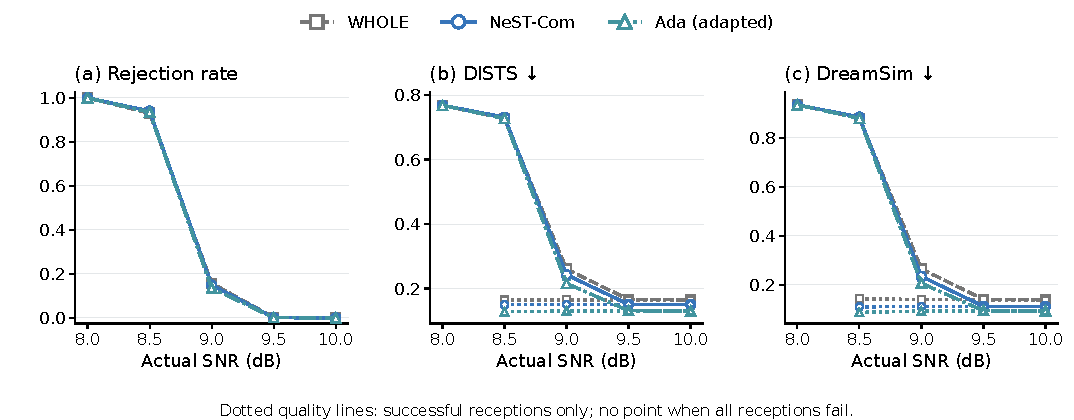
\includegraphics[width=0.92\linewidth]{figures/supp_figure_s2_threshold.pdf}
\caption{Fixed 10-dB transmit policies under downward SNR mismatch. Means and source-bootstrap intervals include gray failures. Dotted quality curves condition on successful receptions and have changing denominators; no such point exists at 8 dB.}\label{fig:threshold}\end{figure}

{\small\setlength{\tabcolsep}{3pt}\renewcommand{\arraystretch}{1.08}
\begin{longtable}{@{}lrrr@{}}\toprule
Actual SNR & WHOLE rejects & NeST rejects & Ada rejects\\\midrule\endhead
8 & 2000 / 2000 & 2000 / 2000 & 2000 / 2000\\*
8.5 & 1861 / 2000 & 1880 / 2000 & 1870 / 2000\\*
9 & 315 / 2000 & 299 / 2000 & 270 / 2000\\*
9.5 & 4 / 2000 & 2 / 2000 & 2 / 2000\\*
10 & 0 / 2000 & 0 / 2000 & 0 / 2000\\
\bottomrule\end{longtable}}
All rejections arise from body/profile parsing; no header rejection, source-decoding rejection or valid NULL frame occurs. All 2000 receptions per method are rejected at 8 dB, whereas none is rejected at 10 dB. The source-cluster intervals retain all 20 realizations of each sampled image. This scan characterizes the tested fixed policies near their threshold, rather than establishing general robustness or low-error-rate operation.
\section{Qualitative examples}\label{sup:6}
The main Fig.3 shows sources 135 and 201 (C10-016/C10-017), selected from the earlier gallery for favorable NeST perceptual reconstructions and retained through unified calibration. WHOLE/NeST/Ada use current 10-dB policies and the first channel repetition, seed 6201; SwinJSCC retains its original first repetition, seed 2001. Full $256\times256$ fields and metrics from the displayed native outputs are retained. These selected cases illustrate possible gains; population comparisons are established by S2, where Ada has lower mean DISTS and DreamSim at 10 dB.

The complementary images below retain their earlier 10-dB configurations. Sources were ranked by mean DISTS gain of Token over WHOLE, with source-index tie breaking and no success filter. Source 209 is the fixed median-rank choice and source 39 the minimum-gain choice, both displayed with the first original repetition. Source 39 worsens in DISTS but improves in DreamSim. Complete source IDs, all five display metrics, and the selected 7-dB advantage examples remain in the companion assets; no sample is reselected in this revision.
\begin{figure}[htbp]\centering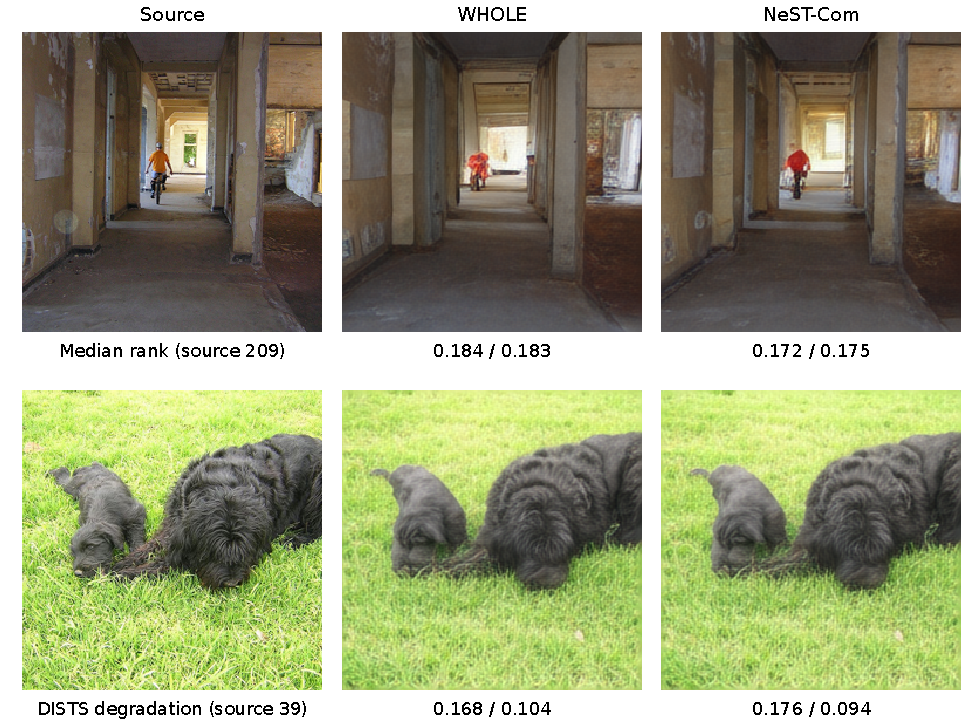
\includegraphics[width=5.8in]{figures/supp_examples_distribution.pdf}
\caption{Median-rank (top) and minimum DISTS-gain (bottom) sources under the earlier $N=1024$, 10-dB policies. Columns are source, WHOLE and NeST. Values are DISTS / DreamSim for the first displayed repetition; lower is favorable.}\label{fig:counterexamples}\end{figure}
\FloatBarrier\section{Processing costs and paired quality}\label{sup:7}
Main timing comparisons use two distinct physical CPU cores on the same RTX PRO 6000 host. Historical measurements used two SMT siblings of one physical core and are retained separately in the companion; the groups are not pooled.
\subsection{Complete TX/RX processing}\label{sup:timing-main}
The first 32 test images use batch one, two warmups and three measurements per image and direction. GPU implementations run serially; BPG uses the same CPU allocation. Timed spans use two intra-op and two inter-op threads. At $N=1024$, 10 dB, token systems use 16-QAM rate 2/3 and WHOLE/NeST/Ada ceilings $(9,0)/(8,126)/256$. These match the current quality experiment's MCS and ceilings, while the directories are earlier versions.

GPU synchronization brackets TX from in-memory RGB to transmitted symbols and RX from received symbols to RGB. Tokenization, condition extraction, CDF/arithmetic coding, independent termination, complete candidate scanning, link processing and reconstruction are included. Model/input loading, final hashing, logging and metric scoring are excluded; BPG retains its source search, codec invocation and RAM serialization. No cached tokens or reconstruction replace timed work. Total processing time is TX plus RX, not radio propagation latency. Means and source-bootstrap intervals (10\,000 resamples) describe this session's image-to-image variation.
\begin{longtable}{@{}lrrl@{}}\toprule
System & TX (ms) & RX (ms) & Total (ms) [95\% CI]\\\midrule\endhead
WHOLE & 215.29 & 366.42 & 581.71 [576.77, 586.78]\\
NeST & 248.44 & 403.99 & 652.43 [647.45, 657.51]\\
Latent & 15.28 & 23.93 & 39.21 [39.20, 39.22]\\
Swin & 21.01 & 18.16 & 39.17 [39.07, 39.30]\\
BPG & 2209.97 & 21.28 & 2231.26 [2163.61, 2298.68]\\
\bottomrule\end{longtable}
\subsection{Matched granularity}\label{sup:timing-grid}
The four grids fix ceiling $(8,126)$, model, MCS and fitting rule. Token shares the identical NeST TX cell; the main WHOLE policy, with its different ceiling, is not substituted for matched Whole. Times include shared scale-wise probability computation, independent termination and full candidate scanning.
\begin{longtable}{@{}lrl@{}}\toprule
Grid & TX (ms) & 95\% source interval\\\midrule\endhead
Whole & 185.20 & [184.76, 185.67]\\
Quarter & 215.84 & [215.33, 216.41]\\
Eighth & 217.76 & [217.18, 218.48]\\
Token & 248.44 & [246.78, 251.06]\\
\bottomrule\end{longtable}
Token costs about 14.1\% more TX time than Eighth and adds 0.066 dB mean PSNR at this matched point (S3). Eighth and Token offer different quality--computation choices. All listed implementations successfully complete their measured receptions.
\subsection{Compiled Ada and its matched output quality}\label{sup:timing-compiled}\label{sup:timing-compiled-quality}
The compiled route uses conditional causal prefill and \texttt{torch.compile}; independent RX reconstructs CDFs from received tokens with the same tensor shape and strict causal mask, using public zeros for unknown future inputs. CFG 4, sampling rules, weights, classifier, tokenizer, decoder, MCS and precision are unchanged. Cold compilation and model loading are excluded; timed spans use the same two physical cores. Compilation itself uses eight cores.
\begin{longtable}{@{}lrl@{}}\toprule
Implementation span & Mean (ms) & 95\% source interval\\\midrule\endhead
TX & 114.55 & [114.15, 114.93]\\
RX & 2949.76 & [2945.89, 2953.91]\\
TOTAL & 3064.30 & [3060.46, 3068.37]\\
\bottomrule\end{longtable}

Prefill/compilation can change floating-point CDFs and bitstreams. Although independent decoding recovers the same source tokens, payload-derived tail seeds can consequently change. The 32-source quality comparison below uses the actual timed outputs and matching original events. All 32 restored outputs match their timed hashes. Fixing the original generation seeds makes all 32 native images identical to the original route; the actual timed outputs differ on 30 sources. Intervals crossing zero do not establish implementation equivalence.

{\small\setlength{\tabcolsep}{3pt}\renewcommand{\arraystretch}{1.08}
\begin{longtable}{@{}lr@{}}\toprule
Metric & Compiled minus original [paired 95\% CI]\\\midrule\endhead
PSNR $\uparrow$ & \cival{-0.038}{-0.471}{0.392}\\
LPIPS $\downarrow$ & \cival{-0.0017}{-0.0052}{0.0018}\\
DreamSim $\downarrow$ & \cival{-0.0035}{-0.0084}{0.0008}\\
CLIP-I $\uparrow$ & \cival{-0.0010}{-0.0061}{0.0038}\\
DISTS $\downarrow$ & \cival{-0.0018}{-0.0044}{0.0009}\\
\bottomrule\end{longtable}}
The compiled outputs have mean PSNR 19.36069, DISTS 0.13098, DreamSim 0.09640, LPIPS 0.16355 and CLIP-I 0.87857. Their paired processing cost is 3064.30 ms (114.55 TX + 2949.76 RX); no new latency is assigned to the fixed-seed control. The 500-image main quality results keep the original implementation. Historical SMT timings, two-source prefill diagnostics, counters and execution history are available in the companion rather than pooled into this comparison.
\section{Transfer to Kodak24}\label{sup:8}
The 24 images use the original RGB center $256\times256$ crop without prior resizing. Models and earlier ImageNet-calibrated policies remain frozen at 4/10/19 dB, with three channel repetitions per image. Quarter and NeST share the target ceilings but use different fallback grids. At 19 dB, historical Ada uses 64-QAM rate 5/6 rather than the current 16-QAM rate 5/6; this tests transfer of the historical configurations, not the current Table IV policy. All receptions are accepted. Statistics average repetitions within each of 24 sources and use the fixed 10\,000-by-24 source bank.

\textbf{All source means.}\par
{\small\setlength{\tabcolsep}{3pt}\renewcommand{\arraystretch}{1.08}
\begin{longtable}{@{}llrrrrr@{}}\toprule
SNR & Method & PSNR $\uparrow$ & DISTS $\downarrow$ & DreamSim $\downarrow$ & LPIPS $\downarrow$ & CLIP-I $\uparrow$\\\midrule\endhead
4 & Ada & 13.533 & 0.2573 & 0.3062 & 0.4544 & 0.7873\\*
4 & Quarter & 18.618 & 0.1947 & 0.1766 & 0.2714 & 0.8384\\*
4 & NeST & 18.790 & 0.1957 & 0.1716 & 0.2605 & 0.8411\\*
4 & WHOLE & 18.223 & 0.2068 & 0.2042 & 0.2903 & 0.8194\\
10 & Ada & 19.924 & 0.1314 & 0.1015 & 0.1739 & 0.8810\\*
10 & Quarter & 21.009 & 0.1568 & 0.1102 & 0.1762 & 0.8692\\*
10 & NeST & 21.130 & 0.1536 & 0.1047 & 0.1716 & 0.8844\\*
10 & WHOLE & 20.335 & 0.1673 & 0.1266 & 0.2029 & 0.8599\\
19 & Ada & 21.464 & 0.1134 & 0.0827 & 0.1408 & 0.8981\\*
19 & Quarter & 22.875 & 0.1271 & 0.0795 & 0.1230 & 0.8955\\*
19 & NeST & 23.052 & 0.1251 & 0.0775 & 0.1187 & 0.8983\\*
19 & WHOLE & 22.647 & 0.1295 & 0.0808 & 0.1269 & 0.8974\\
\bottomrule\end{longtable}}

\textbf{Direct paired differences [95\% CI].}\par
{\small\setlength{\tabcolsep}{3pt}\renewcommand{\arraystretch}{1.08}
\begin{longtable}{@{}llrrrrr@{}}\toprule
SNR & Difference & PSNR $\uparrow$ & DISTS $\downarrow$ & DreamSim $\downarrow$ & LPIPS $\downarrow$ & CLIP-I $\uparrow$\\\midrule\endhead
4 & NeST-Ada & \cival{+5.257}{4.601}{5.934} & \cival{-0.0616}{-0.0749}{-0.0486} & \cival{-0.1346}{-0.1747}{-0.0988} & \cival{-0.1939}{-0.2145}{-0.1742} & \cival{+0.0537}{0.0239}{0.0834}\\*
4 & NeST-Quarter & \cival{+0.172}{0.051}{0.313} & \cival{+0.0010}{-0.0038}{0.0056} & \cival{-0.0050}{-0.0162}{0.0039} & \cival{-0.0108}{-0.0160}{-0.0060} & \cival{+0.0027}{-0.0113}{0.0150}\\*
4 & NeST-WHOLE & \cival{+0.567}{0.395}{0.745} & \cival{-0.0111}{-0.0163}{-0.0059} & \cival{-0.0326}{-0.0467}{-0.0191} & \cival{-0.0298}{-0.0361}{-0.0232} & \cival{+0.0216}{0.0104}{0.0329}\\
10 & NeST-Ada & \cival{+1.206}{0.664}{1.847} & \cival{+0.0221}{0.0120}{0.0312} & \cival{+0.0032}{-0.0132}{0.0161} & \cival{-0.0024}{-0.0142}{0.0086} & \cival{+0.0034}{-0.0176}{0.0257}\\*
10 & NeST-Quarter & \cival{+0.121}{0.072}{0.174} & \cival{-0.0032}{-0.0062}{-0.0004} & \cival{-0.0054}{-0.0096}{-0.0016} & \cival{-0.0047}{-0.0080}{-0.0015} & \cival{+0.0152}{0.0061}{0.0243}\\*
10 & NeST-WHOLE & \cival{+0.794}{0.509}{1.091} & \cival{-0.0138}{-0.0199}{-0.0079} & \cival{-0.0218}{-0.0331}{-0.0110} & \cival{-0.0314}{-0.0422}{-0.0205} & \cival{+0.0245}{0.0132}{0.0378}\\
19 & NeST-Ada & \cival{+1.589}{1.396}{1.781} & \cival{+0.0117}{0.0077}{0.0157} & \cival{-0.0052}{-0.0126}{0.0033} & \cival{-0.0222}{-0.0264}{-0.0184} & \cival{+0.0001}{-0.0126}{0.0142}\\*
19 & NeST-Quarter & \cival{+0.177}{0.122}{0.235} & \cival{-0.0020}{-0.0037}{-0.0006} & \cival{-0.0020}{-0.0036}{-0.0003} & \cival{-0.0044}{-0.0064}{-0.0027} & \cival{+0.0028}{-0.0021}{0.0075}\\*
19 & NeST-WHOLE & \cival{+0.405}{0.307}{0.509} & \cival{-0.0045}{-0.0065}{-0.0026} & \cival{-0.0033}{-0.0055}{-0.0011} & \cival{-0.0082}{-0.0107}{-0.0060} & \cival{+0.0009}{-0.0062}{0.0070}\\
\bottomrule\end{longtable}}
NeST improves PSNR, DISTS and DreamSim over WHOLE at all three SNRs. Against Quarter, DISTS/DreamSim intervals exclude zero at 10/19 dB and cross zero at 4 dB. Against Ada, both distances favor NeST at 4 dB; DISTS favors Ada at 10/19 dB and DreamSim intervals cross zero. The five-metric tables retain these mixed outcomes; complete marginal intervals, other contrasts and source-level distributions are in the companion CSVs.

\end{document}
